Comme nous l’avons expliqué précédemment, la reconnaissance d’émotions est un domaine jeune mais dont la maturité grandissante impliquera des applications diverses, ainsi on retrouve des applications tel que Picxel qui a développé un kit logiciel qui identifie les émotions du visage lorsque l'utilisateur est devant son ordinateur, permettant à la machine de s'adapter en conséquence.

\begin{figure}[htp]
\centering
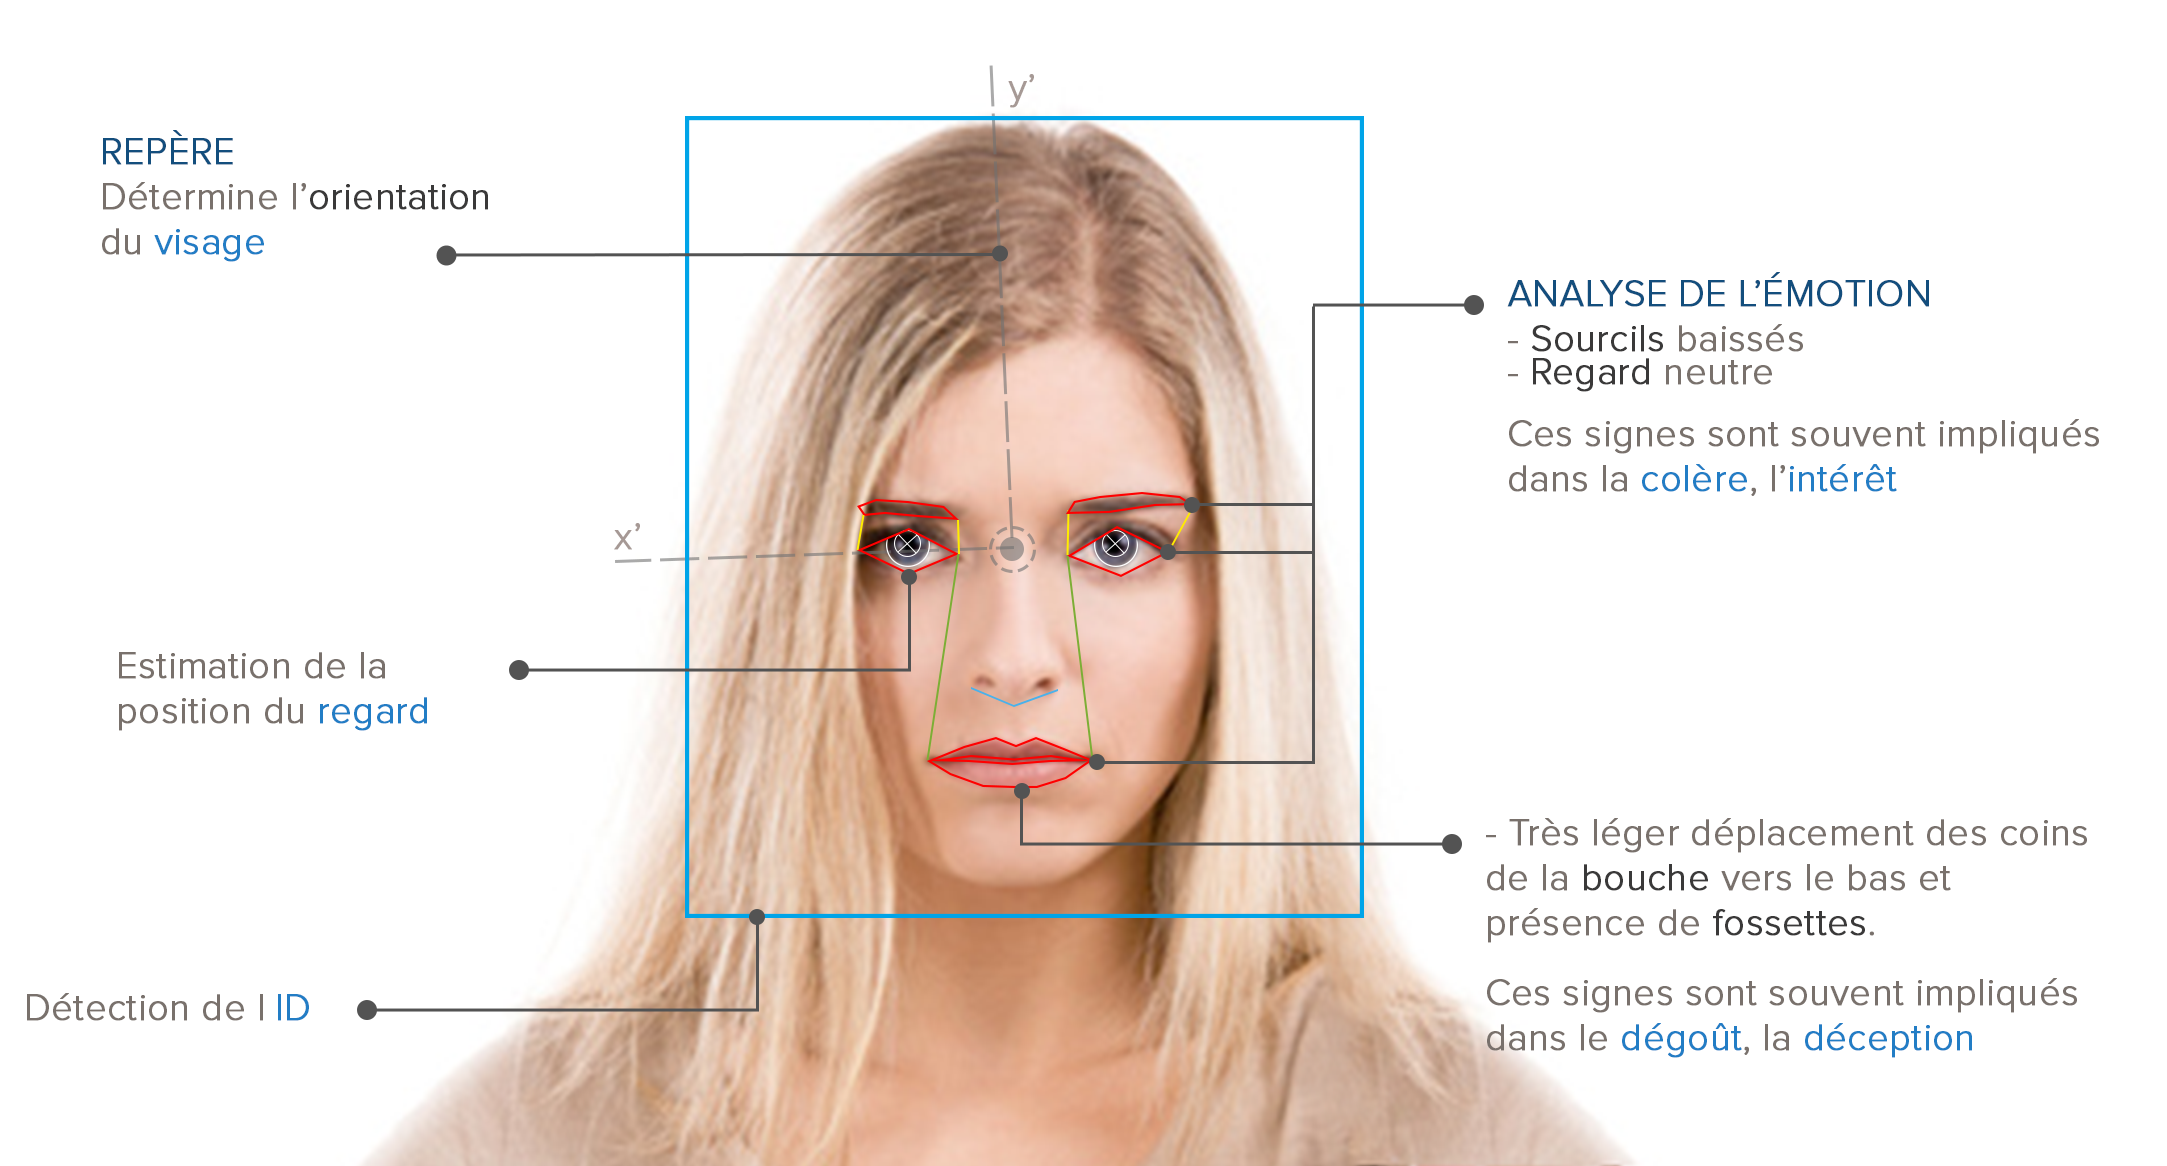
\includegraphics[scale=0.9]{./images/etatArt1.png}
\caption{Image issue de picxel.fr - Illustration de la colère}
\label{eA1}
\end{figure}

On retrouve également la société Beyond Verbal qui a lancé une application qui permet d’extraire, de décoder et de mesurer un spectre d’émotion à partir de la voix brute d’une personne.
Ou encore une application pour Google Glass baptisée Emotient qui permettra à l’utilisateur d’obtenir des informations sur les émotions de son interlocuteur.\\

Par ailleurs, la classification de l’émotion générée par la musique n’est pas quelque chose de nouveau, en effet on retrouve des services web tel que Musicovery qui effectue une classification des musiques sur un repère orthogonal avec deux axes : calme-énergétique et sombre-positif (Cf figure \ref{eA2}).

\begin{figure}[htp]
\centering
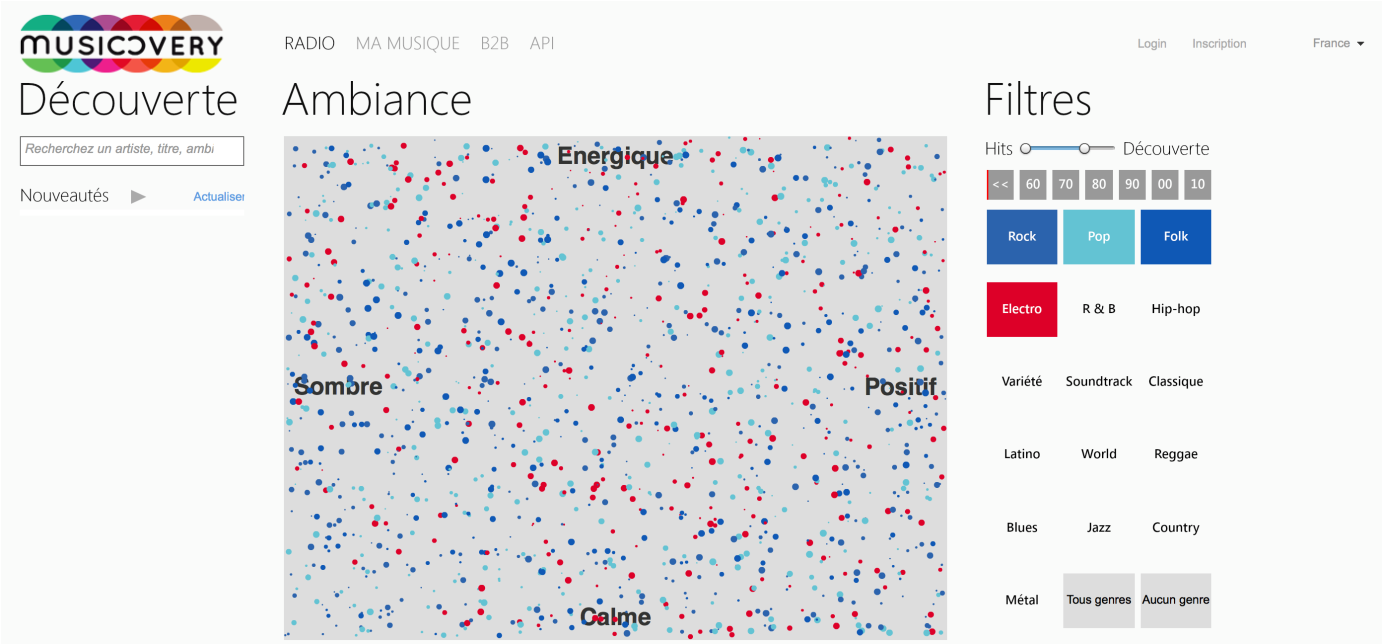
\includegraphics[scale=1.0]{./images/etatArt2.png}
\caption{Capture d'écran du site de streaming Musicovery}
\label{eA2}
\end{figure}

Dans un genre proche, certains sites de streaming ou applications tels que \emph{Stereomood} ou \emph{Moodflow} permettent d'accéder à une playlist correspondant à une émotion.
Cependant, dans ce cas c'est à l'utilisateur de choisir la playlist qu'il doit écouter, en cherchant donc dans un premier temps à identifier sa propre émotion.
De plus les musiques proposées par ces deux services sont celles d'une certaine base de musiques sur internet, et pas les musiques de l'utilisateur.

De même, l'analyse des goûts musicaux à partir de playlists, à travers une classification automatique se retrouve dans certains projets récents tel que \textit{Prizm}, lancé par une startup française et dont la commercialisation doit commencer début 2016.
C'est un objet diffusant de la musique choisie automatiquement, en fonction des goûts des utilisateurs et de l'ambiance de la pièce où il se trouve.
De plus il devient de plus en plus “intelligent” à mesure qu'on interagit avec lui.
Cela fournit un exemple de recommandation en fonction de paramètres extérieurs, et non juste selon un filtrage collaboratif, auquel sont limités les sites de streaming.
Ainsi ce processus de machine learning pourra également être utilisé dans le cadre de la classification automatique de nos musiques.

\begin{figure}[htp]
\centering
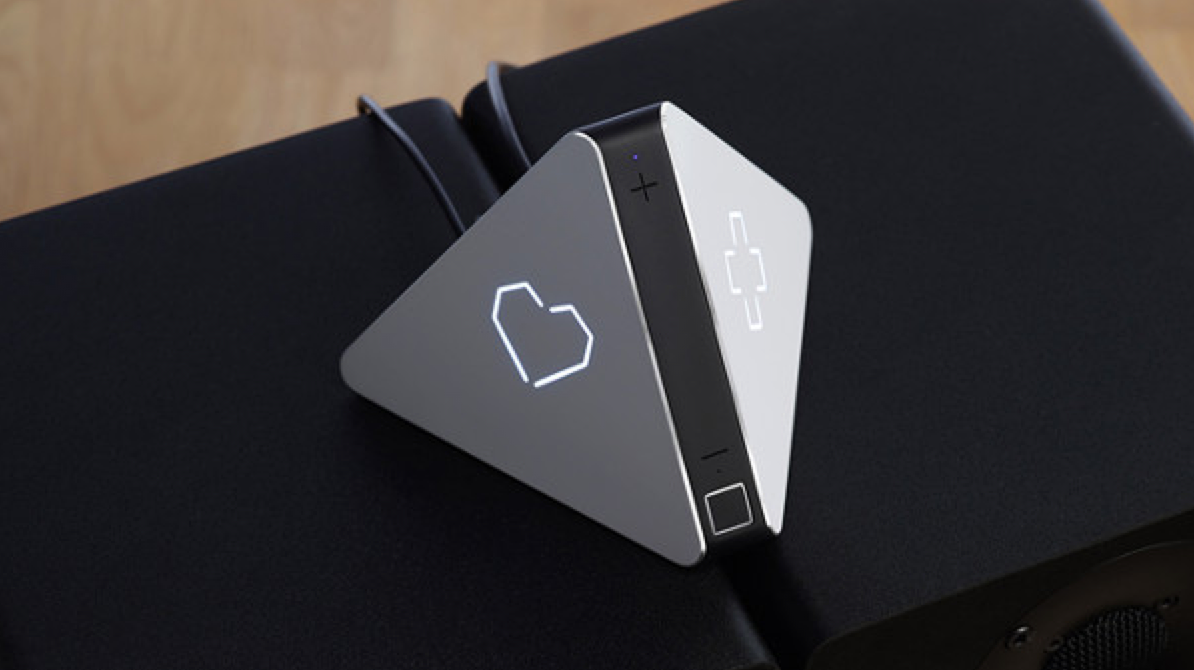
\includegraphics[scale=0.70]{./images/etatArt3.png}
\caption{Boîtier de Prizm}
\end{figure}

Il restera donc, dans le cadre de notre projet, à construire ce « pont » qui nous permettra de relier l’émotion ressentie par l’utilisateur et l’ambiance suscitée par la musique, ce qui marquera le côté innovant de notre projet.
